\lab{Algorithms}{The Finite Element method}{The Finite Element method}
\label{lab:FEM}
Recall that the heat equation is given by
\begin{align*}
y_t = \epsilon y_{xx} + f(x) %\label{FEM:diffusion}
\end{align*}
where $f(x)$ represents any heat sources in the system, and $\epsilon y_{xx}$ models the diffusion of heat.
Suppose we wish to study the distribution of heat in a fluid that is moving at some constant speed $a$.
We can model this by adding an advection term to the heat equation, giving us
\begin{align*}
y_t + ay_x = \epsilon y_{xx} + f(x).
\end{align*}
This fluid flows through a pipe from $x = 0$ to $x = 1$ at a speed $a = 1$, and as it travels it is warmed a constant rate $f= 1$.
Suppose also that $y = 2$ at $x = 0$, so that the fluid is already at a constant temperature as it enters the pipe.

As time increases we expect the temperature of the fluid in the pipe to reach a steady state distribution; this heat distribution would then satisfy the ODE
\begin{align}
\begin{split}
&{ } \epsilon y'' - y' = -1,\\
&{ } y(0) = 2.
\end{split}\label{eqn:FEM_steady_state}
\end{align}
At the moment this problem is not fully defined, since the ODE is second order and there is only one boundary condition.
Suppose a device is installed on the end of the pipe that nearly instantaneously brings the heat of the water up to $y = 4$.
Physically we expect this extra heat that is introduced at $x = 1$ to diffuse backward through the water in the pipe.

We will use the finite element method to solve this boundary value problem numerically.

\begin{figure}[ht]
\centering
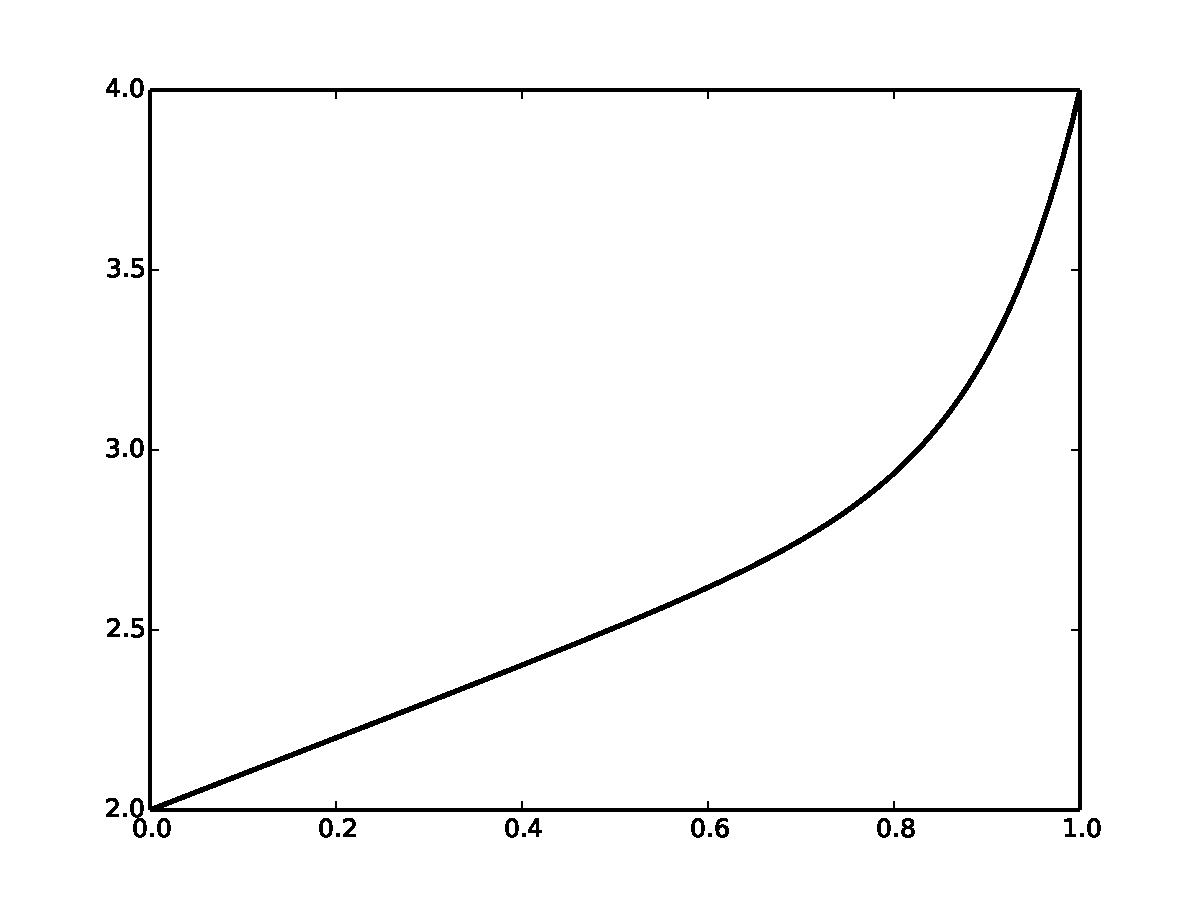
\includegraphics[width=\textwidth]{FEM_solution.pdf}
\caption{The analytic solution of \eqref{eqn:FEM_steady_state} when $\epsilon = .1$, with the additional condition that $y(1) = 4$.}
\label{fig:FEM_analytic_solution}
\end{figure}

\section*{The Weak Formulation}
Consider the equation
\begin{align}
	\begin{split}
	&{ }\epsilon y'' - y' = -1,\\
	&{ }y(0) = \alpha, \quad y(1) = \beta .
	\end{split}\label{eqn:FEM_eqn1}
\end{align}
To find the solution $y$ using the finite element method, we reframe the problem and look at what is known as its weak formulation.

%We may assume that the solution $y$ of \eqref{eqn:FEM_eqn1} lies in some appropriate function space $V$.
%; in any case, we can approximate it arbitrarily well in $C^0[0,1]$ by a piecewise linear function.
Let $w$ be a smooth function on $[0,1]$ satisfying $w(0) = w(1) = 0$.
Multiplying \eqref{eqn:FEM_eqn1} by $w$ and integrating over $[0,1]$ yields
\begin{align*}
	\int_0^1 f w &= \int_0^1 \epsilon y''w - y'w, \\
	&= \int_0^1 -\epsilon y'w' - y'w.
\end{align*}
Define a bilinear function $a$ and a linear function $l$ by
\begin{align*}
a(y,w) &= \int_0^1 -\epsilon y'w' - y'w,\\
l(w) &= \int_0^1 f w.
\end{align*}
Rather than trying to solve \eqref{eqn:FEM_eqn1}, we instead consider the problem of finding a function $y$ such that
\begin{align}
	a(y,w) &= l(w), \quad \forall \, w \in V_0,
	\label{eqn:FEM_integral_form}
\end{align}
where $V$ is some appropriate vector space that is expected to allow us to approximate the solution $y$, and $V_0 = \{w \in V|w(0) = w(1) = 0\}$.
(For example, we could consider the space of functions that are piecewise linear with vertices at a fixed set of points.
This example is discussed further below.)
This equation is called the weak formulation of \eqref{eqn:FEM_eqn1}.

Let $\mathrm{P}_n$ be some partition of $[0,1]$, $0 = x_0 < x_1< \ldots < x_{n} = 1$, and let $V_n$ be the finite-dimensional vector space of continuous functions $v$ on $[0,1]$ where $v$ is linear on each subinterval $[{x_j,x_{j+1}}]$.
These subintervals are the finite elements for which this method is named.
$V_n$ has dimension $n+1$, since there are $n+1$ degrees of freedom for continuous piecewise linear functions in $V$.
Let $V_{n0}$ be the subspace of $V_n$ of dimension $n-1$ whose elements are zero at the endpoints of $[0,1]$, and let $\triangle x_n = \max_{0 \leq j \leq n-1}|x_{j+1} - x_j|$.

Let $\{\mathrm{P}_n\}$ be a sequence of partitions that are refinements of each other, such that $\triangle x_n \to 0$ as $n \to \infty$.
Then in particular $V_1 \subset V_2 \subset \ldots \subset V_n \ldots \subset V$.
For each partition $\mathrm{P}_n$ we can look for an approximation $y_n \in V_n$ for the true solution $y$; if this is done  correctly then $y_n \to y$ as $n \to \infty$.

\section*{The Numerical Method}
Consider a partition $\mathrm{P}_5 = \{x_0, x_1, \ldots, x_5\}$.
We will define some basis functions $\phi_i$, $i = 0, \ldots, 5$ for the corresponding vector space $V_5$.
Let the $\phi_i$ be the hat functions 
\[\phi_i(x) = \begin{cases}
(x - x_{i-1})/h_i \quad \quad\text{ if } x \in [x_{i-1},x_i]\\
 (x_{i+1} - x)/h_{i+1} \quad \text{ if } x \in [x_{i},x_{i+1}]\\
0 \quad \quad \quad \quad \quad \quad \quad \,\,\text{ otherwise}
\end{cases}\]
where $h_i = x_i - x_{i-1}$; see Figures \ref{fig:FEM_one_basis_function} and \ref{fig:FEM_basis_functions}. 

\begin{figure}[ht]
\centering
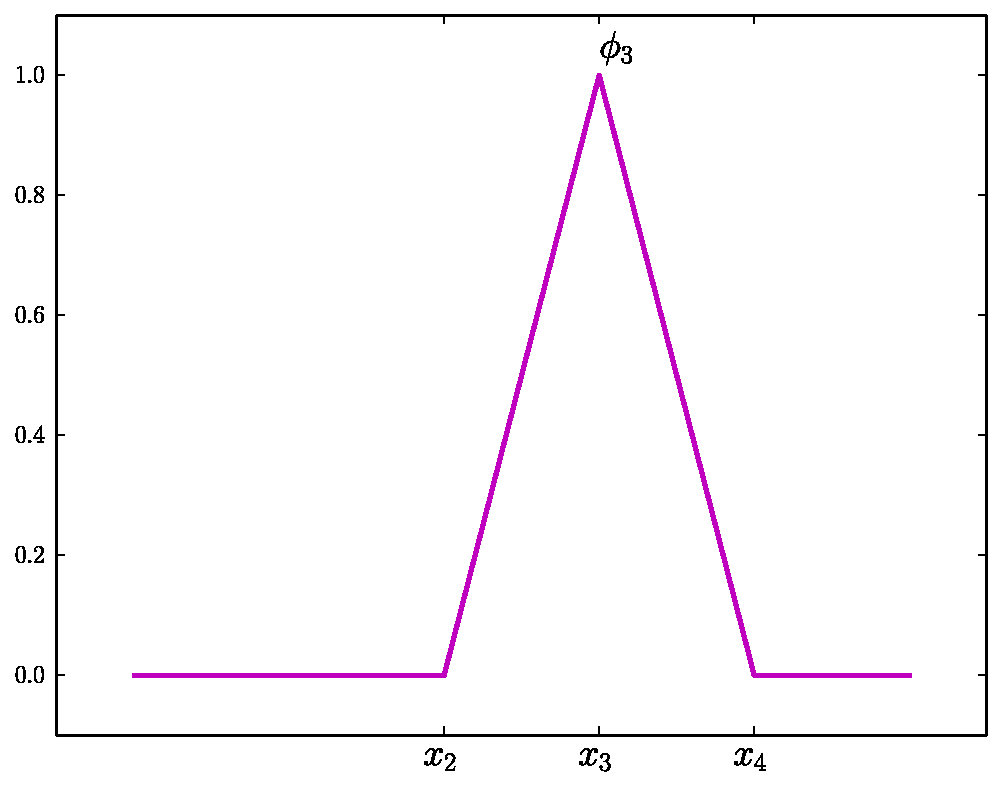
\includegraphics[width=\textwidth]{one_basis_function.pdf}
\caption{The basis function $\phi_3$.}
\label{fig:FEM_one_basis_function}
\end{figure}

\begin{figure}[ht]
\centering
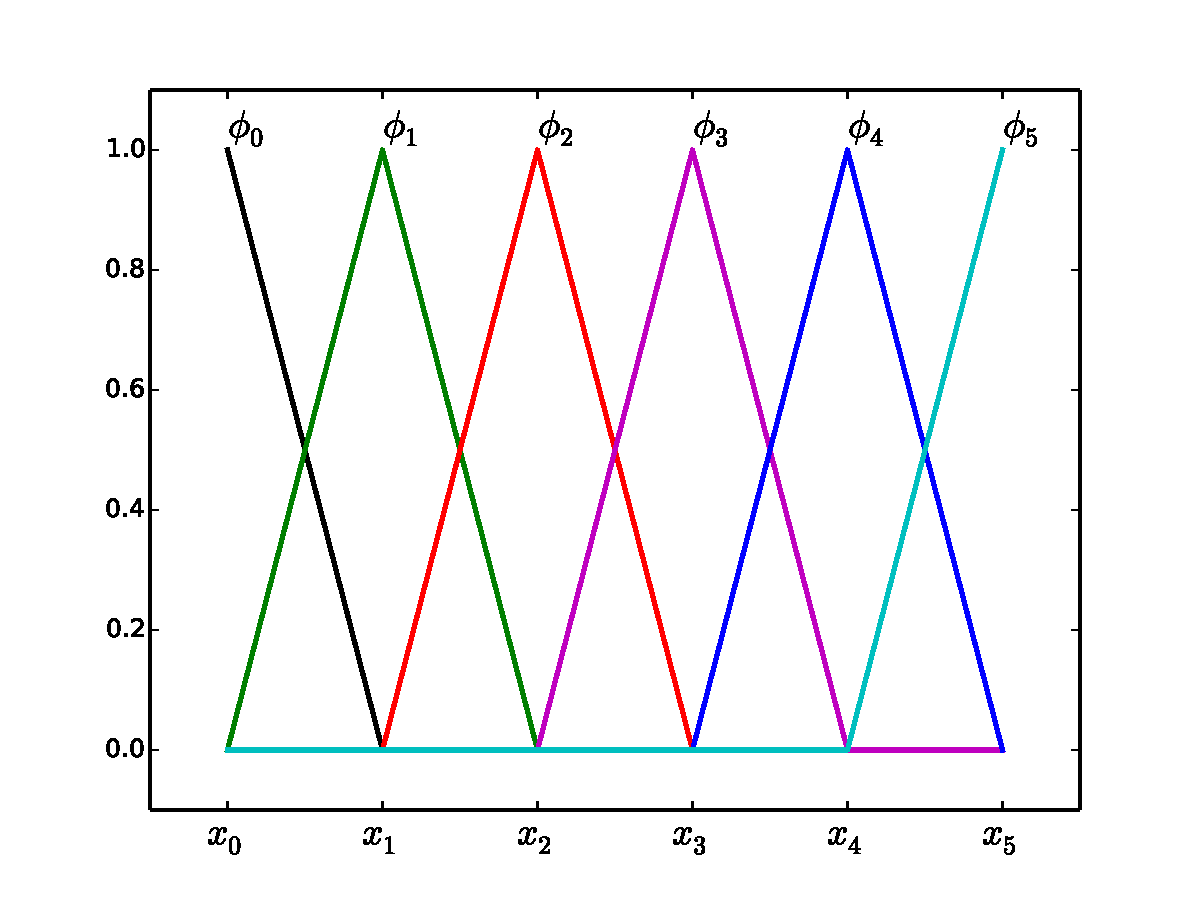
\includegraphics[width=\textwidth]{basis_functions.pdf}
\caption{Basis functions for $V_5$.}
\label{fig:FEM_basis_functions}
\end{figure}

We look for an approximation $\hat{y} = \sum_{i=0}^5 k_i \phi_i \in V_5$ of the true solution $y$; to do this we must determine appropriate values for the constants $k_i$.
We impose the condition on $\hat{y}$ that 
\[a(\hat{y},w) = l(w) \quad \forall \, w \in V_{50}.\]
Equivalently, we require that 
\[a \left( \sum_{i=0}^5 k_i \phi_i,\phi_j \right) = l(\phi_j) \quad \text{for } j = 1,2,3,4,\]
since $\phi_1, \phi_2, \phi_3, \phi_4$ form a basis for $V_{50}$.

Since $a$ is bilinear, we obtain 
\[\sum_{i=0}^5 k_i  a ( \phi_i,\phi_j ) = l(\phi_j) \quad \text{for } j = 1,2,3,4.\]
To satisfy the boundary conditions, we also require that $k_0 = \alpha$, $k_5 = \beta$.
These equations can be written in matrix form as
\begin{align} AK = \Phi,\label{eqn:FEM_linear_system}\end{align}
where
\[A = \left[\begin{array}{cccccc}1 & 0 & 0 & 0 & 0 & 0 \\a(\phi_0,\phi_1) & a(\phi_1,\phi_1) & a(\phi_2,\phi_1) & 0 & 0 & 0 \\0 & a(\phi_1,\phi_2) & a(\phi_2,\phi_2) & a(\phi_3,\phi_2) & 0 & 0 \\0 & 0 & a(\phi_2,\phi_3) & a(\phi_3,\phi_3) & a(\phi_4,\phi_3) & 0 \\0 & 0 & 0 & a(\phi_3,\phi_4) & a(\phi_4,\phi_4) & a(\phi_5,\phi_4) \\0 & 0 & 0 & 0 & 0 &1\end{array}\right]\]
and
\[K = \left[\begin{array}{c}k_0 \\k_1 \\k_2 \\k_3 \\k_4 \\k_5\end{array}\right] , \quad\Phi =  \left[\begin{array}{c}\alpha \\l(\phi_1) \\l(\phi_2) \\l(\phi_3) \\l(\phi_4) \\\beta\end{array}\right].\]

Note that $a(\phi_i,\phi_j) = 0$ for most values of $i, j$ (that is, when the hat functions do not have overlapping domains).
Thus the finite element method results in a sparse linear system.
To compute the coefficients of \eqref{eqn:FEM_linear_system} we begin by evaluating some integrals.
Since
\[\phi_i'(x) = \begin{cases}
1/h_i \quad \quad \quad \, \text{for } x_{i-1} < x < x_i,\\
 -1/h_{i+1} \quad \text{ for } x_{i} < x < x_{i+1},\\
0 \quad \quad \quad \quad \, \text{ otherwise},
\end{cases}\]
we obtain
\begin{align*}
\int_0^1  \phi_i'\phi_j' &= \begin{cases}
- 1/h_{i+1} \quad \quad \quad \text{ if } j=i+1,\\
1/h_i + 1/h_{i+1} \quad \text{if } j=i,\\
0 \quad \quad \quad \quad \quad \quad \, \text{ otherwise},
\end{cases} \\
\int_0^1  \phi_i'\phi_j &= \begin{cases}
- 1/2 \quad \,\text{ if } j=i+1,\\
1/2 \quad \quad \text{ if } j=i-1,\\
0 \quad \quad \quad \text{ otherwise},
\end{cases} \\
a(\phi_i,\phi_j) &= \begin{cases}
\epsilon/h_{i+1} + 1/2 \quad \quad \, \text{ if } j=i+1,\\
-\epsilon/h_i -\epsilon/h_{i+1} \quad  \text{ if } j=i,\\
\epsilon/h_i - 1/2 \quad \quad \quad \, \text{ if } j=i-1,\\
0 \quad \quad \quad \quad \quad \quad \,\,\,\,\,\,\, \text{ otherwise},
\end{cases}\\
l(\phi_j) &= -(1/2)(h_j + h_{j+1}).
\end{align*}
\eqref{eqn:FEM_linear_system} may now be solved using any standard linear solver.

In this case, in order to handle the large number of elements required for Problem \ref{prob:FEM_accuracy_comparison}, you will want to use the tridiagonal algorithm provided in several of the earlier labs (for example Lab \ref{lab:finitedifference1}), or the banded matrix solver included in \li{scipy.linalg}.

\begin{problem}
Use the finite element method to solve
\begin{align}
	\begin{split}
	&{ }\epsilon y'' - y' = -1,\\
	&{ }y(0) = \alpha, \quad y(1) = \beta,
	\end{split} \label{eqn:FEM_exercise}
\end{align}
where $\alpha = 2, \beta = 4$, and $\epsilon = 0.02$.
Use $N = 100$ finite elements ($101$ grid points).
Compare your solution with the analytic solution
\[y(x) = \alpha + x + (\beta - \alpha - 1 ) \frac{e^{x/\epsilon} -1}{e^{1/\epsilon} -1}.\]

\eqref{eqn:FEM_exercise} is a singularly perturbed ODE, so-named because the parameter $\epsilon$ is a coefficient of the highest order derivative in the equation.
The character of the problem changes dramatically when $\epsilon = 0$: since the limit equation (as $\epsilon \to 0$) is first-order, it only allows for one boundary condition.
Thus as $\epsilon$ gets smaller, the rightmost boundary condition is satisfied at the `last moment',  and cannot be satisfied when $\epsilon = 0$.
\end{problem}

\begin{problem}
One of the strengths of the finite element method is the ability to generate grids that better suit the problem.
In two dimensions the finite elements are quadrilaterals and triangles, and can be used to approximate irregular domains.
The finite element method can also be used to solve PDEs where the shape and size of the domain changes over time.

The solution of \eqref{eqn:FEM_exercise} changes most rapidly near $x = 1$.
Compare the numerical solution when the grid points are unevenly spaced versus when the grid points are clustered in the area of greatest change. Specifically, use the grid points defined by
\begin{lstlisting}
even_grid = np.linspace(0,1,6)
clustered_grid = np.linspace(0,1,6)**(1./8)
\end{lstlisting}
What is the difference in accuracy?
\end{problem}

% \begin{figure}[ht]
% \centering
% \includegraphics[width=\textwidth]{FEM_singular_solution.pdf}
% \caption{The analytic solution of \eqref{FEM:exercise}.}
% \label{FEM:analytic_solution}
% \end{figure}

\begin{problem}
\label{prob:FEM_accuracy_comparison}
Higher order methods promise faster convergence, but typically require more work to code.
So why do we use them when a low order method will converge just as well, albeit with more grid points?
The answer concerns the roundoff error associated with floating point arithmetic.
Low order methods generally require more floating point operations, so roundoff error has a much greater effect.

The finite element method introduced here is a second order method, even though the approximate solution is piecewise linear.
(To see this, note that if the grid points are evenly spaced, the matrix $A$ in \eqref{eqn:FEM_linear_system} is exactly the same as the matrix for the second order centered finite difference method.)

Solve \eqref{eqn:FEM_exercise} with the finite element method using $N = 2^i$  finite elements, $i = 4, 5, \ldots, 21$.
Use a log-log plot to graph the error.
Then find the error when using the pseudospectral method and the same number of grid points.
What do you see?
\end{problem}

% \begin{align}
% \left[\begin{array}{cccccc}1 & 0 & 0 & 0 & 0 & 0 \\-\epsilon/h_1 & \epsilon/h_1 + \epsilon/h_2 & -\epsilon/h_2 & 0 & 0 & 0 \\0 & -1/h_2 & a(\phi_2,\phi_2) & a(\phi_3,\phi_2) & 0 & 0 \\0 & 0 & a(\phi_2,\phi_3) & a(\phi_3,\phi_3) & a(\phi_4,\phi_3) & 0 \\0 & 0 & 0 & a(\phi_3,\phi_4) & a(\phi_4,\phi_4) & a(\phi_5,\phi_4) \\0 & 0 & 0 & 0 & 0 &1\end{array}\right]
% \left[\begin{array}{c}k_0 \\k_1 \\k_2 \\k_3 \\k_4 \\k_5\end{array}\right] = \left[\begin{array}{c}\alpha \\l(\phi_1) \\l(\phi_2) \\l(\phi_3) \\l(\phi_4) \\\beta\end{array}\right] \label{FE:linear_system}
% \end{align}

\section*{A Comparison of Numerical Methods}

\begin{center}
  \begin{tabular}{ l |l l }
    % \hline
     & Finite Element & Finite Difference  \\ \hline
    Linear System& sparse& sparse  \\
   Derivative & approximated locally & approximated locally \\
Domain & irregular domains & fairly regular\\
% Problem Formulation & integral & derivative & derivative & integral \\
Convergence & polynomial & polynomial \\
Strengths & adaptive mesh & easier to understand \\
& refinement & and implement \\
& complex geometries & easier for higher dimensions \\
    \hline
  \end{tabular}
\end{center}

\begin{center}
  \begin{tabular}{ l |l l }
    % \hline
      & Pseudospectral & Finite Volume \\ \hline
    Linear System & dense & sparse \\
   Derivative & global & local\\
Domain  & very nice & fairly regular\\
Convergence  & exponential & polynomial\\
Strengths  & fast convergence & handling discontinuities in \\
& accurate to high precisions &the initial conditions \\
& & dealing with shock formation \\
& & and propagation \\
    \hline
  \end{tabular}
\end{center}

It is important to note that these methods are often mixed, so, for example, it is common to work with a finite element mesh in space and a finite differencing scheme in time.